%%
%% The MIT License (MIT)
%%
%% Copyright (c) 2016 Matthias Fischer
%%
%% Permission is hereby granted, free of charge, to any person obtaining a copy
%% of this software and associated documentation files (the "Software"), to deal
%% in the Software without restriction, including without limitation the rights
%% to use, copy, modify, merge, publish, distribute, sublicense, and/or sell
%% copies of the Software, and to permit persons to whom the Software is
%% furnished to do so, subject to the following conditions:
%% 
%% The above copyright notice and this permission notice shall be included in all
%% copies or substantial portions of the Software.
%% 
%% THE SOFTWARE IS PROVIDED "AS IS", WITHOUT WARRANTY OF ANY KIND, EXPRESS OR
%% IMPLIED, INCLUDING BUT NOT LIMITED TO THE WARRANTIES OF MERCHANTABILITY,
%% FITNESS FOR A PARTICULAR PURPOSE AND NONINFRINGEMENT. IN NO EVENT SHALL THE
%% AUTHORS OR COPYRIGHT HOLDERS BE LIABLE FOR ANY CLAIM, DAMAGES OR OTHER
%% LIABILITY, WHETHER IN AN ACTION OF CONTRACT, TORT OR OTHERWISE, ARISING FROM,
%% OUT OF OR IN CONNECTION WITH THE SOFTWARE OR THE USE OR OTHER DEALINGS IN THE
%% SOFTWARE.
%%

% save old roman pagecount and set the number format to arabic
\setcounter{myPageRomanCounter}{\value{page}}
\pagenumbering{arabic}

\section{Einleitung}
\label{sec:Einleitung}
\blindtext
\begin{figure}[h]
	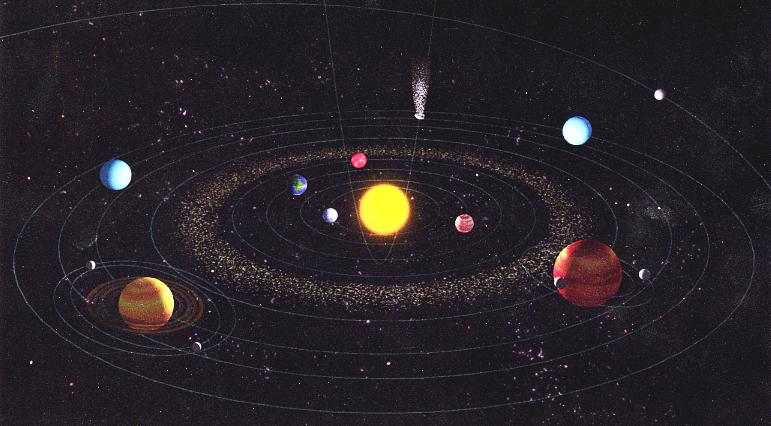
\includegraphics[width=\textwidth]{solar_bad.jpg}
	\caption{Das Sonnensystem}
	\label{fig:das-sonnensystem}
\end{figure}
	
\section{Einsatzfeld}
\label{sec:Einsatzfeld}
\blindtext 
Blablabla\footnote{\cite[S.~20]{Reim.2015}}

\blindtext 

\section{Theoretischen Grundlagen}
\label{sec:Theorie}
\blindtext
Hallo dies ist ein Test.\footnote{\cite[S.~428]{Reim.2015}}

\begin{table}
	\begin{tabularx}{\textwidth}{X X X X}
		\toprule
		Data1 		& Data2 	& Data3		& Data4 \\
		\midrule
		Some data 	& Some data & Some data & Some data \\
		Some data 	& Some data & Some data & Some data \\
		Some data 	& Some data & Some data & Some data \\
		Some data 	& Some data & Some data & Some data \\
		\bottomrule
	\end{tabularx}
	\caption{Einige Daten}
	\label{tab:test-table}
\end{table}

\blindtext

\section{Übertragung auf die betriebliche Praxis}
\label{sec:Praxis}
\blindtext

\subsection{Teil 1}
\label{subsec:Teil1}
\blindtext

\subsection{Teil 2}
\label{subsec:Teil2}
\blindtext

\section{Kritische Reflexion}
\label{sec:Kritik}
\blindtext

\section{Fazit}
\label{sec:Fazit}
\blindtext

% draw page
\clearpage
% change numberformat and set the old roman counter
\pagenumbering{Roman}
\setcounter{page}{ \value{myPageRomanCounter} }